\chapter{Implementation Scenario}
 \begin{figure}[!htbp]
	\centering
	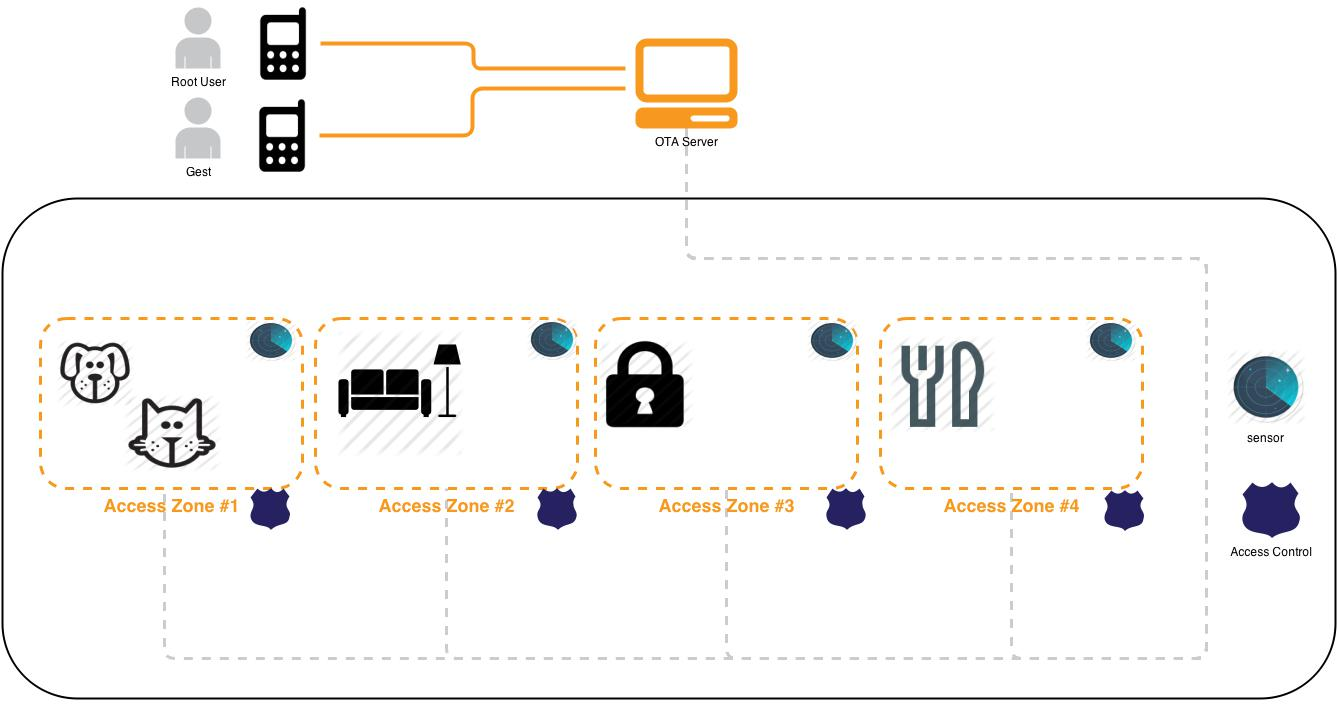
\includegraphics[width=1\textwidth]{homeoverview.jpg}
		\caption{Smart Home}
	\label{fig:SmartHome}
\end{figure}

\section{Overview}
Figure~\ref{fig:SmartHome} describes the basic structure and functionalities provided by implementation scenario Smart Home.
In the above-mentioned housing scenario, embedded with UICC smart card sensors which are in charge of monitoring and reporting environment variables, such as, home temperature, luminance and how much water the pet has, as well as embedded UICC smart card electronic device, for instance coffee maker, are deployed. On each this sensor and device an OPC UA server is installed, whose major responsibilities are controlling that corresponding device as well as processing data gathered by it.  Moreover each door in this scenario is equipped with a digital lock, that only allows user with enough authority to access. This electronic lock is also integrated an smart card and installed the OPC UA server application. Users in this scenario can be householder or guests of home owner. Using cell phone with UICC smart card and on this mobile terminal installed OPC UA client application, subscriber is capable of configuring sensors and querying data gathered by sensors, remote controlling aforementioned secure devices, viewing historical information recorded by corresponding facilities. With the help of such services a comfortable living condition is created in an automated way.  Moreover the root user, namely the owner of this house, is also able to assign the permission of accessing particular room to other guests. In case of when he/she is taking a vocation and pet cannot get necessary care.


In this implementation scenario, OPC UA clients, namely Universal Integrated Circuit Card (UICC)  based phone user communicates with OPC UA server, which is deployed on other secure hard devices, via an OTA server.   Smart card that is applied in this scenario acts as security token for both OPC UA client and server and it contains credential information like encryption keys. certificates and digital signature. The communication stack, that manages secure  communication between OPC UA client and server application, is also developed and integrated on smart card as a Java Card applet, which means without corresponding UICC card, OPC UA client and server are not able to appropriately finish their work.


 \begin{figure}[ht]

	\centering
	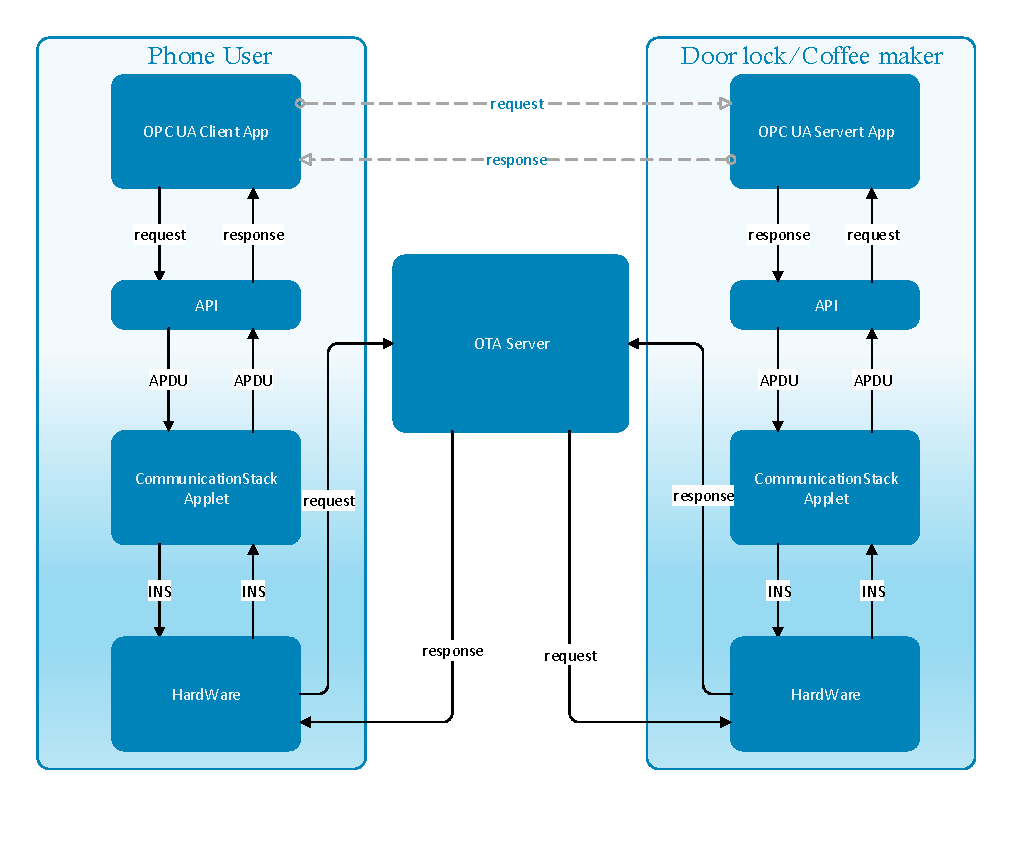
\includegraphics[width=1.1\textwidth]{csoverview}
		\caption{OPC UA Client Server Structure Example}
	\label{fig:softwareStructure}
\end{figure}


\section {Software Structure}
Figure~\ref{fig:softwareStructure} pictures aforementioned OPC UA client server structure. OP UA Client and Server application communicate with each other with the help of an OTA server. And the communication stack,  is in charge of creation and managing the secure communication between OTA server and secure device. Moreover using different chip card, OPC UA client application is able to communicate with OPC UA server application using Short Message Service(SMS) or TCP/IP based web service. 
\newline
server on secure device provides following services:
 \begin{itemize}
  \item processing client subscription/publishing environment data
  \item secure message exchange with client
  \item authority management
  \item historical data record
  \item execution client's command
\end{itemize}
Basic client functions as following are provided:
 \begin{itemize}
  \item submitting subscription/receiving published data
  \item secure message exchange with server
  \item sending command/configuration data
  \item providing user friendly interface
\end{itemize}

Communication stack is integrated in UICC smart card, whose responsibility is realizing secure channel as well as session management, transporting data to receiver using TCP/IP connections. An internal API translates OPC UA application instructions in to Application Protocol Data Unity (APDU) messagse and forwards them to smart card OS, which is eventually in charge of user authentication and processing secure messaging between card application and chip card pair. 

Moreover thanks to self-containment structure, smart card itself does not dependent on other external resources, which could be extreme vulnerable to potential secure attack, and therefore provides a better hardware security and OS security.

 \begin{figure}
	\centering
	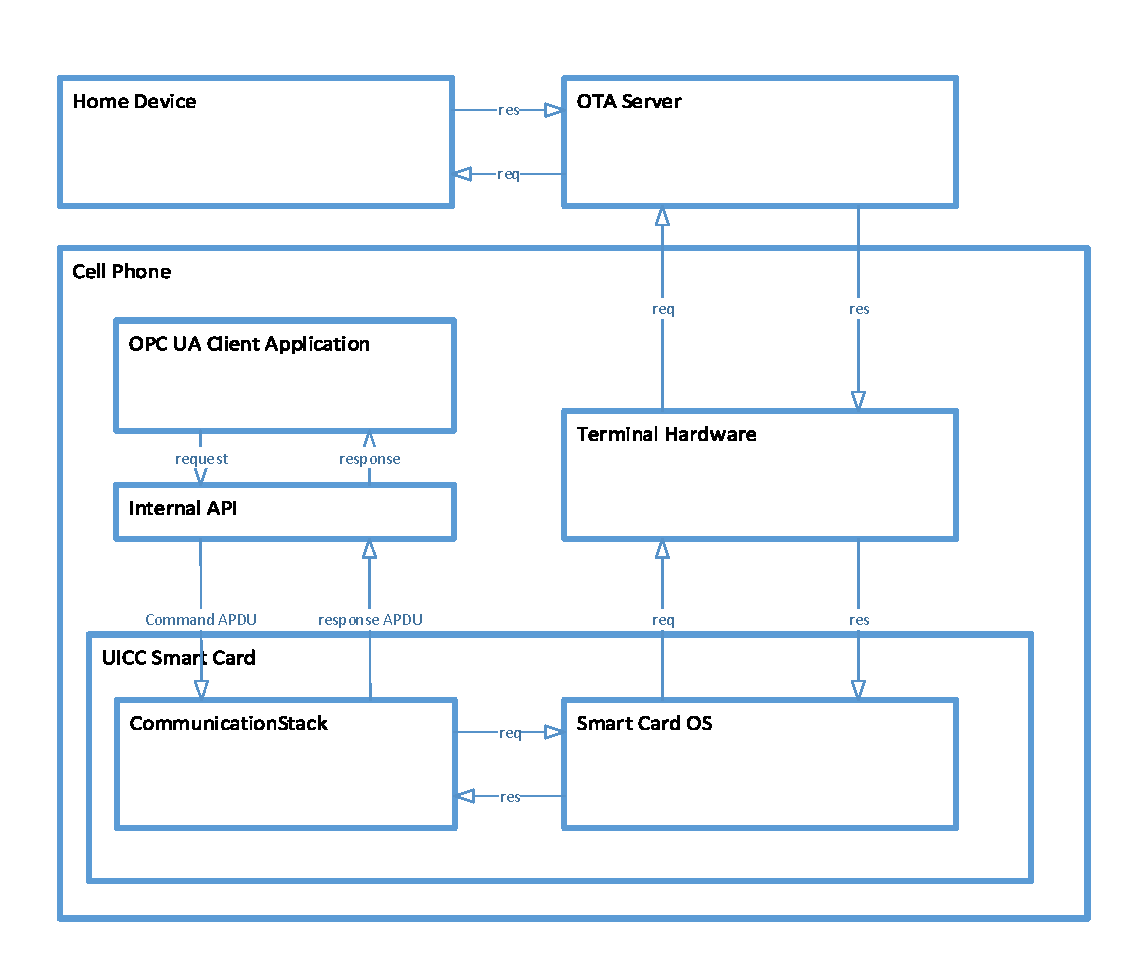
\includegraphics[width=1.2\textwidth]{clientStructure}
		\caption{Client Structure}
	\label{fig:clientStructure}
\end{figure}
\subsection{Client Structure}
As described in figure~\ref{fig:clientStructure}, the OPC UA client consists of client application code that realizes client application level functions, OPC UA client API that translates client application instructions into APDU and forwards APDU to UICC smart card as well as  manages secure communication between smart card and OPC UA client application code, which is realized as Android  App. The Communication stack is developed and integrated with UICC card and its main responsibilities are:
\begin{itemize}
  \item initiate HTTP session based on TLS(proactive)
  \item trigger HTTP session based on trigger SMS send by OTA server(passive)
  \item rebuild broken communication channel
  \item message encryption as well as decryption
  \item message transmit
\end{itemize}

\begin{figure}
	\centering
	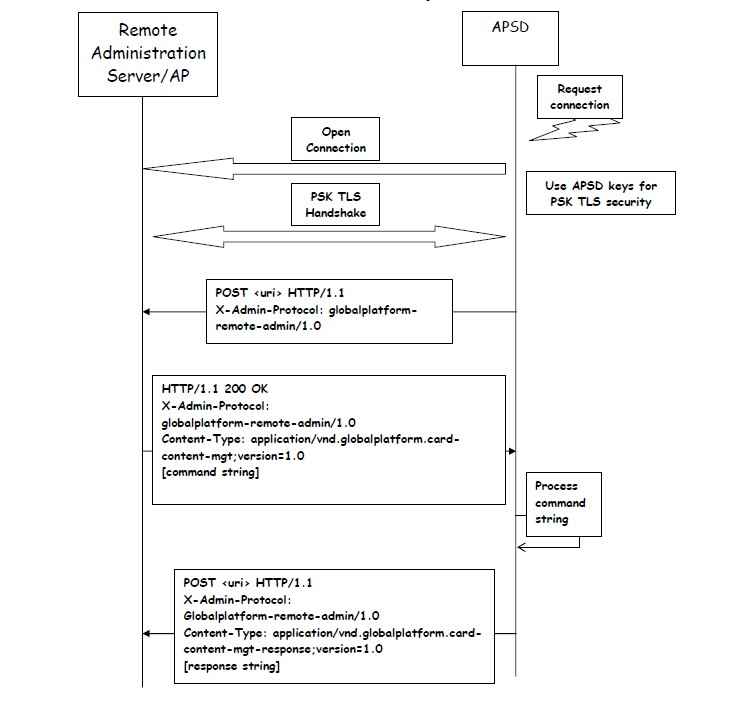
\includegraphics[width=1.2\textwidth]{apsd.jpg}
		\caption{Communication Flow between an AP and corresponding APSD\cite{ramGP}}
	\label{fig:apsd}
\end{figure}
The communication flow compliant with the one provided by GlobalPlatform, which provides mechanisms that allow secure information exchanged between a remote entity and a terminal, this process is also known as Remote Application Management(RAM) over HTTP protocol and PSK TLS security. The on card component, which is responsible for connection creation with the remote entity and user/application authentication, is called Security Domain(SD). And the aforementioned remote entity  is  referred as Remote Administration Server as well. With these concepts, smart card with Security Domain issued  by GloablPlatform can act as HTTP client and is capable of packing APDU formate information into HTTP POST message and transmitting HTTP message to OTA server, which will then forward this HTTP message to target receiver.\cite{ramGP}
 
Figure~\ref{fig:apsd} illustrates a typical communication flow between administration server and corresponding security domain (Application Security Domain) on smart card. As can be seen, the request for open communication is usually initialized by security domain, which is also the phone user. After a successful creation of secure handshake, the remote administration server and security domain is able to use HTTP connection to exchange request and response strings, which include APDU instructions. GlobalPlatform has also provided  a lists of API used to initialize authentication process, to configure algorithm and keys for message  encryption and decryption, to perform message exchange  behavior and so on.

\subsection{Server Structure}

\begin{figure}
	\centering
	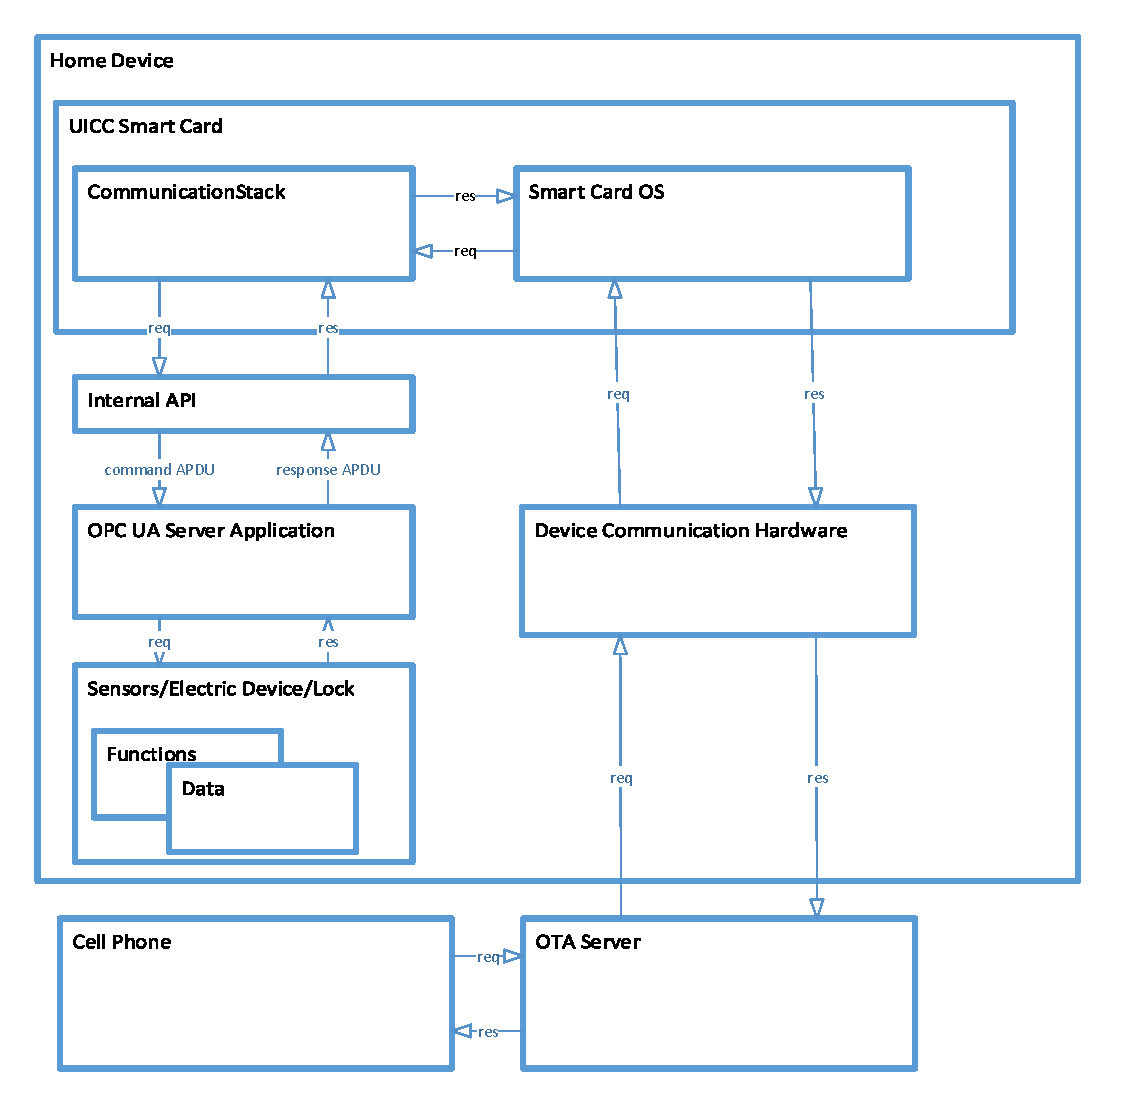
\includegraphics[width=1.2\textwidth]{serverStructure}
		\caption{Server Structure}
	\label{fig:serverStructure}
\end{figure}
Server here refers sensors, electric device as well digital locks that together build up the smart home system. Each server controls exactly one above-mentioned secure device and take subscription as well as publish corresponding notification to authenticated subscriber. The server structure is pictured as figure~\ref{fig:serverStructure} and it consists of OPC UA server application code, which offers basic server like subscription and notification mentioned before, an internal API and a on smart card integrated communication stack.

\subsection{Implementation Tool Support}
Morpho presents JACADE with full name, Java Card Applet Develop Environment, which is more than just a IDE but a complex selection of various class API and software modules, that can be applied to design complete Java Card Applet as well as to debug Java source. When it comes to running test with Java Card Applet, apart from using regular cell phone with UICC smart card, on where to be tested applet is installed, Morpho Card Reader (MCR) or Java virtual card together with iCardReader, Universal Test Environment (UTE) can be applied. To be more specifically, iCardReader is a tool developed by Morpho and be used in order to send APDU script to Java virtual card or to real smart card connected with test PC using smart card reader such as MCR reader, and to monitor corresponding response APDU information. Universal Test Environment provided by Morpho uses Java languages developed test cases and test scenarios\footnote{Test scenario is a collection of relative test cases.} to simulate user cases and obverse related smart card reactions. In contrast with iCardreader, which can only send APDU command sequence to smart card, UTE integrates more software models that can be used to simulate such as security domain offered by other card application provider, and therefore can provide more sophisticate test environment.